% This LaTeX was auto-generated from MATLAB code.
% To make changes, update the MATLAB code and export to LaTeX again.

\documentclass{article}

\usepackage[utf8]{inputenc}
\usepackage[T1]{fontenc}
\usepackage{lmodern}
\usepackage{graphicx}
\usepackage{color}
\usepackage{hyperref}
\usepackage{amsmath}
\usepackage{amsfonts}
\usepackage{epstopdf}
\usepackage[table]{xcolor}
\usepackage{matlab}

\sloppy
\epstopdfsetup{outdir=./}
\graphicspath{ {./topt_p3_antonio_fernandez_andres_herencia_images/} }

\matlabhastoc

\begin{document}

\label{T_B44F81CE}
\matlabtitle{\textbf{PRACTICE 3 - NONLINEAR OPTIMIZATION WITH CONSTRAINTS}}

\begin{par}
\begin{flushleft}
\textbf{Andrés Herencia y Antonio Fernández}
\end{flushleft}
\end{par}

\begin{par}
\begin{flushleft}
\textbf{MUTECI 2023-2024}
\end{flushleft}
\end{par}

\matlabtableofcontents{Table of Contents}

\label{H_D7D67F5B}
\matlabheading{\textbf{Exercise 1}}

\begin{par}
\begin{flushleft}
For the following nonlinear problem
\end{flushleft}
\end{par}

\begin{par}
\begin{flushleft}
\includegraphics[width=\maxwidth{25.388861013547416em}]{image_0}
\end{flushleft}
\end{par}

\begin{par}
\begin{flushleft}
It is requested
\end{flushleft}
\end{par}

\begin{par}
\begin{flushleft}
a. Determine the KKT points. 
\end{flushleft}
\end{par}

\begin{par}
\begin{flushleft}
b. Identify the optimum from the previous points. 
\end{flushleft}
\end{par}

\begin{par}
\begin{flushleft}
c. Use MATLAB (or any other software) to identify the optimum starting from various points, for example, (-0.5, -0.5); (0.5, 0.5); (2, 1) and verify if the same solution is reached. 
\end{flushleft}
\end{par}

\begin{par}
\begin{flushleft}
d. Perform two iterations with the Zoutendijk algorithm starting from the point (2, 1).
\end{flushleft}
\end{par}


\label{H_F989F904}
\matlabheadingtwo{Solution}

\begin{par}
\begin{flushleft}
Before starting to compute, we can represent the function to make some interpretations about the solution.
\end{flushleft}
\end{par}

\begin{matlabcode}
clear; clc; clf;

f = @(x1,x2) 2.*x1 - x2;
g1 = @(x1,x2) -x1.^2 + x2 <=0;
g2 = @(x1,x2) x1.^2 - 2.*x1 + 1 + x2 - 5 <=0;
g3 = @(x1,x2) -x2 <= 0;

[Xgrid,Ygrid]=meshgrid(-5:0.01:5,-5:0.01:5);
z = f(Xgrid,Ygrid); z1 = g1(Xgrid,Ygrid); z2 = g2(Xgrid,Ygrid); z3 = g3(Xgrid,Ygrid);

fig1 = figure(1);
surface(Xgrid,Ygrid,z,'EdgeColor','none','FaceAlpha',0.8)
hold on
s1 = surface(Xgrid,Ygrid,z1,'FaceColor','[0 0.4470 0.7410]', ...
    'FaceAlpha',0.3, 'EdgeColor','none');
s2 = surface(Xgrid,Ygrid,z2,'FaceColor','[0.8500 0.3250 0.0980]', ...
    'FaceAlpha',0.3, 'EdgeColor','none');
s3 = surface(Xgrid,Ygrid,z3,'FaceColor','[0.4660 0.6740 0.1880]', ...
    'FaceAlpha',0.3, 'EdgeColor','none');
hold off
grid on
title('f(x_1,x_2)')
xlabel('x_1')
ylabel('x_2')
view([-45 -45])
legend('f(x1,x2','g1(x1,x2)','g2(x1,x2)','g3(x2)')

view([-45 45])
\end{matlabcode}
\begin{center}
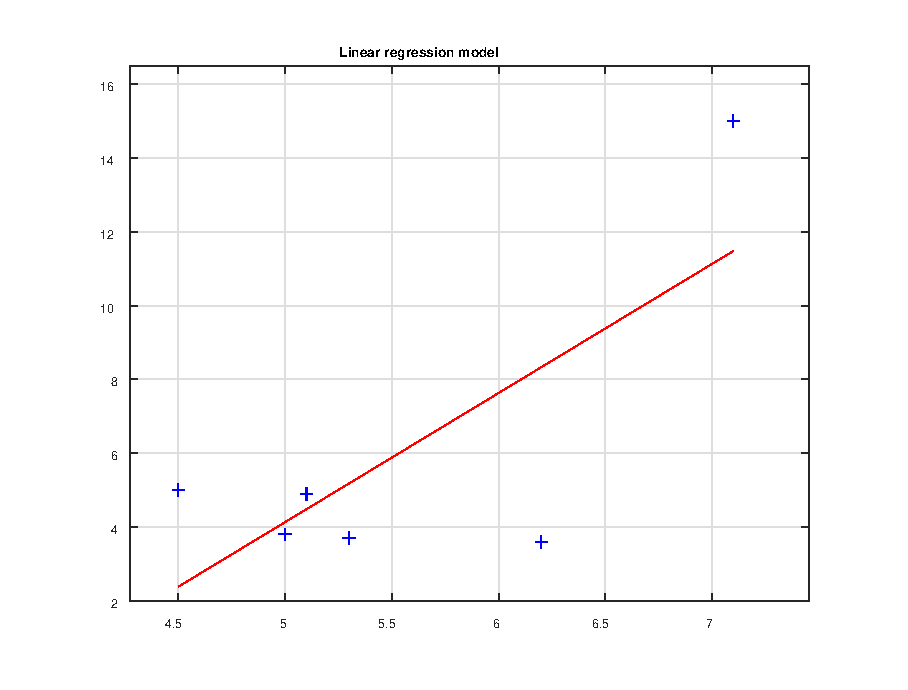
\includegraphics[width=\maxwidth{56.196688409433015em}]{figure_0.eps}
\end{center}


\label{H_3122655C}
\matlabheadingthree{a) Determine the KKT points. }

\begin{par}
\begin{flushleft}
We will compute te KKT points.
\end{flushleft}
\end{par}

\begin{matlabcode}
syms x1 x2 u1 u2 u3;

obj = 2.*x1 -x2;
ineq1 = -x1.^2 + x2;
ineq2 = (x1 - 1).^2 + x2 - 5;
ineq3 = -x2;

L = obj + u1*ineq1 +u2*ineq2 +u3*ineq3;
dL_dx1 = diff(L, x1);
dL_dx2 = diff(L, x2);

eq1 = dL_dx1 == 0;
eq2 = dL_dx2 == 0;
eq3 = u1*ineq1 == 0;
eq4 = u2*ineq2 == 0;
eq5 = u3*ineq3 == 0;

sol = solve([eq1, eq2, eq3, eq4, eq5], [x1, x2, u1, u2, u3]);

KKTpoints = [];

for i = 1:length(sol.x1)

    x1_sol = sol.x1(i);
    x2_sol = sol.x2(i);
    u1_sol = sol.u1(i);
    u2_sol = sol.u2(i);
    u3_sol = sol.u3(i);

    if subs(ineq1, [x1, x2], [x1_sol,x2_sol])<=0 && ...
        subs(ineq2, [x1, x2], [x1_sol,x2_sol])<=0 && ...
        subs(ineq3, [x1, x2], [x1_sol,x2_sol])<=0
        if u1_sol >= 0 && u2_sol >= 0 && u3_sol >= 0
            KKTpoints = [KKTpoints; [x1_sol, x2_sol]];
        end
    end
end

disp(KKTpoints)
\end{matlabcode}
\begin{matlabsymbolicoutput}
\hskip1em $\displaystyle \left(\begin{array}{cc}
1 & 1\\
-1 & 1\\
2 & 4
\end{array}\right)$
\end{matlabsymbolicoutput}


\label{H_7C06EA93}
\matlabheadingthree{b) Identify the optimum from the previous points. }

\begin{par}
\begin{flushleft}
We evaluate the function at each point and check when it achieves the lowest value.
\end{flushleft}
\end{par}

\begin{matlabcode}
subs(obj, [x1, x2], [KKTpoints(1,1),KKTpoints(1,2)])
\end{matlabcode}
\begin{matlabsymbolicoutput}
ans = 

\hskip1em $\displaystyle 1$
\end{matlabsymbolicoutput}
\begin{matlabcode}
subs(obj, [x1, x2], [KKTpoints(2,1),KKTpoints(2,2)]) % minimum value
\end{matlabcode}
\begin{matlabsymbolicoutput}
ans = 

\hskip1em $\displaystyle -3$
\end{matlabsymbolicoutput}
\begin{matlabcode}
subs(obj, [x1, x2], [KKTpoints(3,1),KKTpoints(3,2)])
\end{matlabcode}
\begin{matlabsymbolicoutput}
ans = 

\hskip1em $\displaystyle 0$
\end{matlabsymbolicoutput}

\begin{par}
\begin{flushleft}
\textbf{The optimum from the previous points is }$\left(-1,1\right)\;$\textbf{ with value }$-3\ldotp$
\end{flushleft}
\end{par}

\begin{par}
\begin{flushleft}
We can represent the points in a figure
\end{flushleft}
\end{par}

\begin{matlabcode}
fig1;
hold on
plot3(1, 1, f(1,1),'ro','LineWidth',3);
plot3(-1, 1, f(-1,1),'ko','LineWidth',3);
plot3(2, 4, f(2,4),'bo','LineWidth',3);

view([-40.8 6.0])
legend('f(x1,x2','g1(x1,x2)','g2(x1,x2)','g3(x2)','[1,1]','[-1,1]','[2,4]')

view([-90 90])
\end{matlabcode}
\begin{center}
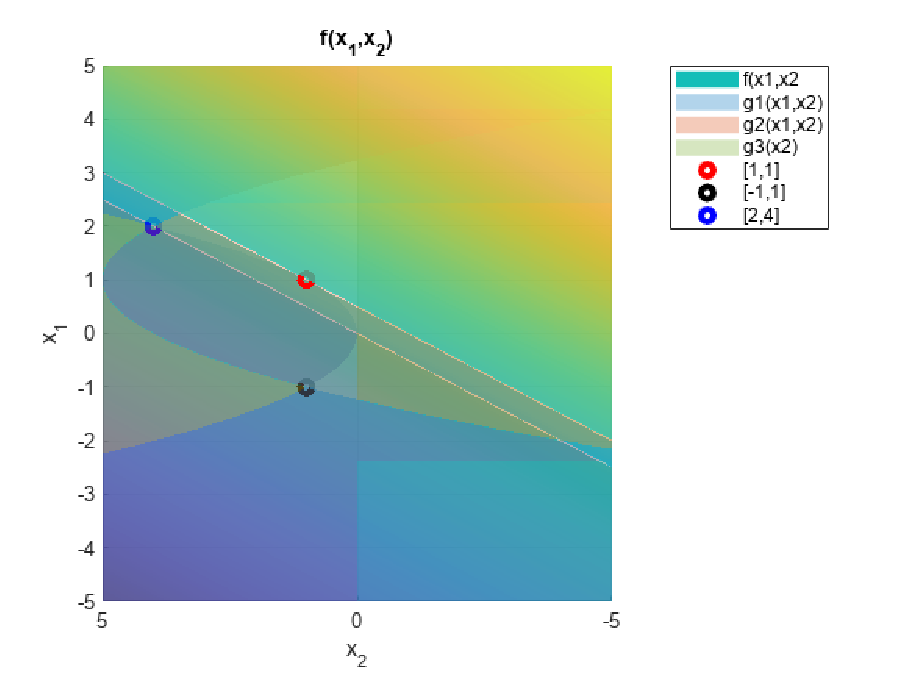
\includegraphics[width=\maxwidth{56.196688409433015em}]{figure_1.eps}
\end{center}


\label{H_F658B924}
\matlabheadingthree{c) Use MATLAB (or any other software) to identify the optimum starting from various points, for example, \texttt{(-0.5, -0.5)};\texttt{ (0.5, 0.5)}; \texttt{(2, 1)} and verify if the same solution is reached. }

\begin{par}
\hfill \break
\end{par}

\begin{matlabcode}
x0 = [-0.5 ; -0.5];
lb = [-inf, 0]
\end{matlabcode}
\begin{matlaboutput}
lb = 1x2    
  -Inf     0

\end{matlaboutput}
\begin{matlabcode}
[x,fun,exitflag, output]=fmincon(@top_ejem_pnl_obj,x0,[],[],[],[],lb,[],@top_ejem_pnl_res);
\end{matlabcode}
\begin{matlaboutput}
Local minimum found that satisfies the constraints.

Optimization completed because the objective function is non-decreasing in 
feasible directions, to within the value of the optimality tolerance,
and constraints are satisfied to within the value of the constraint tolerance.

<stopping criteria details>
\end{matlaboutput}
\begin{matlabcode}
x % optimum achieved
\end{matlabcode}
\begin{matlaboutput}
x = 2x1    
           -1
            1

\end{matlaboutput}
\begin{matlabcode}
x0 = [0.5 ; 0.5];
[x,fun,exitflag, output]=fmincon(@top_ejem_pnl_obj,x0,[],[],[],[],lb,[],@top_ejem_pnl_res);
\end{matlabcode}
\begin{matlaboutput}
Local minimum possible. Constraints satisfied.

fmincon stopped because the size of the current step is less than
the value of the step size tolerance and constraints are 
satisfied to within the value of the constraint tolerance.

<stopping criteria details>
\end{matlaboutput}
\begin{matlabcode}
x % nearly [0,0], not a feasible point
\end{matlabcode}
\begin{matlaboutput}
x = 2x1    
   0.00060024
   2.4034e-07

\end{matlaboutput}

\begin{par}
\begin{flushleft}
This is almost [0,0].
\end{flushleft}
\end{par}

\begin{matlabcode}
x0 = [2 ; 1];
[x,fun,exitflag, output]=fmincon(@top_ejem_pnl_obj,x0,[],[],[],[],lb,[],@top_ejem_pnl_res);
\end{matlabcode}
\begin{matlaboutput}
Local minimum found that satisfies the constraints.

Optimization completed because the objective function is non-decreasing in 
feasible directions, to within the value of the optimality tolerance,
and constraints are satisfied to within the value of the constraint tolerance.

<stopping criteria details>
\end{matlaboutput}
\begin{matlabcode}
x % a kkt point
\end{matlabcode}
\begin{matlaboutput}
x = 2x1    
            2
            4

\end{matlaboutput}

\begin{par}
\begin{flushleft}
Depending on the starting point, we get different solutions. This is due to the set of constraints of \textbf{our} \textbf{problem is not convex}, which means that the function can have more than one minimum, so we can not guarantee that we will achieve the global minimum when a local minimum is found. In these types of problems, the algorithm is extremely sensitive to the initial point. Additionally, as the convergence of the problem is difficult, we generally require specific algorithms for its resolution. For these type of problems, we could use the \href{https://www.mathworks.com/products/global-optimization.html}{Global Optimization Toolbox} or another external solver such as \href{https://www.artelys.com/solvers/knitro/}{Knitro}, but it is not the aim of this practice.
\end{flushleft}
\end{par}

\begin{par}
\begin{flushleft}
NOTE: all the \texttt{top\_ejem\_pnl} functions can be found on \hyperref[H_4F795C9E]{annexes}.
\end{flushleft}
\end{par}


\label{H_8AC0C030}
\matlabheadingthree{d) Perform two iterations with the Zoutendijk algorithm starting from the point [\texttt{2, 1]}.}

\begin{par}
\begin{flushleft}
All the own-made function can be found in \hyperref[H_C6BA4E20]{annexes}.
\end{flushleft}
\end{par}

\begin{par}
\begin{flushleft}
\textbf{First iteration}
\end{flushleft}
\end{par}

\begin{matlabcode}
x0 = [2, 1]
\end{matlabcode}
\begin{matlaboutput}
x0 = 1x2    
     2     1

\end{matlaboutput}
\begin{matlabcode}
%Active restrictions
restrictions = {ineq1, ineq2, ineq3};

for i = 1:numel(restrictions)
    result = round(subs(restrictions{i}, [x1, x2], x0),4);
    if result == 0
        disp(['The constraint ', num2str(i), ' is equal to zero.']);
    else
        disp(['The constraint ', num2str(i), ' is not equal to zero.']);
    end
end
\end{matlabcode}
\begin{matlaboutput}
The constraint 1 is not equal to zero.
The constraint 2 is not equal to zero.
The constraint 3 is not equal to zero.
\end{matlaboutput}
\begin{matlabcode}
grad = gradient(obj, [x1, x2])
\end{matlabcode}
\begin{matlabsymbolicoutput}
grad = 

\hskip1em $\displaystyle \left(\begin{array}{c}
2\\
-1
\end{array}\right)$
\end{matlabsymbolicoutput}
\begin{matlabcode}
A = [-1,2,-1; 0,1,0; 0,0,1; 0,-1,0; 0,0,-1];
c = [1;0;0];
b = [0;1;1;1;1];

lb(1:3)=-Inf;

x=linprog(c,A,b,[],[],lb);
\end{matlabcode}
\begin{matlaboutput}
Optimal solution found.
\end{matlaboutput}
\begin{matlabcode}
display(x)
\end{matlabcode}
\begin{matlaboutput}
x = 3x1    
    -3
    -1
     1

\end{matlaboutput}

\begin{par}
\begin{flushleft}
As $z=-3<0\;$then $\left(-1,1\right)$ is a descent direction.
\end{flushleft}
\end{par}

\begin{matlabcode}
xp = 0;
lb = 0;
[l,fun,flag]=fmincon(@top_ejem_pnl_obj2,xp,[],[],[],[],lb,[],@top_ejem_pnl_res2);
\end{matlabcode}
\begin{matlaboutput}
Local minimum found that satisfies the constraints.

Optimization completed because the objective function is non-decreasing in 
feasible directions, to within the value of the optimality tolerance,
and constraints are satisfied to within the value of the constraint tolerance.

<stopping criteria details>
\end{matlaboutput}
\begin{matlabcode}
display(l)
\end{matlabcode}
\begin{matlaboutput}
l = 
      0.69722

\end{matlaboutput}
\begin{matlabcode}
xk1=x0+l*[x(2),x(3)]
\end{matlabcode}
\begin{matlaboutput}
xk1 = 1x2    
       1.3028       1.6972

\end{matlaboutput}

\begin{par}
\begin{flushleft}
The first iteration give us $x_1 =\left(1\ldotp 3028,1\ldotp 6972\right)$.
\end{flushleft}
\end{par}

\begin{par}
\begin{flushleft}
\textbf{Second iteration}
\end{flushleft}
\end{par}

\begin{matlabcode}
for i = 1:numel(restrictions)
    result = round(subs(restrictions{i}, [x1, x2], xk1),4);
    if result == 0
        disp(['The constraint ', num2str(i), ' is equal to zero.']);
    else
        disp(['The constraint ', num2str(i), ' is not equal to zero.']);
    end
end
\end{matlabcode}
\begin{matlaboutput}
The constraint 1 is equal to zero.
The constraint 2 is not equal to zero.
The constraint 3 is not equal to zero.
\end{matlaboutput}
\begin{matlabcode}
gradienterest = gradient(ineq1, [x1, x2]);
A = [-1,2,-1;-1,-2*xk1(1),1;0,1,0;0,0,1;0,-1,0;0,0,-1];
c = [1;0;0];
b = [0;0;1;1;1;1];

lb(1:3)=-Inf;

x=linprog(c,A,b,[],[],lb);
\end{matlabcode}
\begin{matlaboutput}
Optimal solution found.
\end{matlaboutput}
\begin{matlabcode}
display(x)
\end{matlabcode}
\begin{matlaboutput}
x = 3x1    
     -0.13148
      0.43426
            1

\end{matlaboutput}

\begin{par}
\begin{flushleft}
As $z=-0\ldotp 1315<0\;$then $\left(0\ldotp 4343,1\right)$ is a descent direction.
\end{flushleft}
\end{par}

\begin{matlabcode}
xp = 0;
lb = 0;
[l,fun,flag]=fmincon(@top_ejem_pnl_obj3,xp,[],[],[],[],lb,[],@top_ejem_pnl_res3);
\end{matlabcode}
\begin{matlaboutput}
Local minimum found that satisfies the constraints.

Optimization completed because the objective function is non-decreasing in 
feasible directions, to within the value of the optimality tolerance,
and constraints are satisfied to within the value of the constraint tolerance.

<stopping criteria details>
\end{matlaboutput}
\begin{matlabcode}
display(l)
\end{matlabcode}
\begin{matlaboutput}
l = 
       1.9655

\end{matlaboutput}
\begin{matlabcode}
xk2=xk1+l*[x(2),x(3)]
\end{matlabcode}
\begin{matlaboutput}
xk2 = 1x2    
       2.1563       3.6627

\end{matlaboutput}

\begin{par}
\begin{flushleft}
Since the local minimum in that region is located at $\left(2,4\right)$, it seems that $\left(2\ldotp 1563,3\ldotp 6627\right)$ is a good result.
\end{flushleft}
\end{par}


\label{H_C7A7DB30}
\matlabheading{Exercise 2}

\begin{par}
\begin{flushleft}
For the following linear programming problem:
\end{flushleft}
\end{par}

\begin{par}
\begin{flushleft}
\includegraphics[width=\maxwidth{24.184646261916708em}]{image_1}
\end{flushleft}
\end{par}

\begin{par}
\begin{flushleft}
Perform two iterations with the primal-dual interior-point algorithm, either by hand or by programming, whichever is more convenient.
\end{flushleft}
\end{par}


\label{H_D10930AA}
\matlabheadingtwo{Solution}

\begin{par}
\begin{flushleft}
The \texttt{primaldual} function is given in the \hyperref[H_72206DD4]{annexes}.
\end{flushleft}
\end{par}

\begin{matlabcode}
A=[-1,2;2,1];
b=[4;6];
c=[-1;-1];

sol = primaldual(A, b, c, 0.001, 0.9, 0.1, 2);
display(sol);
\end{matlabcode}
\begin{matlaboutput}
sol = 2x1    
        3.912
        5.112

\end{matlaboutput}


\label{H_E0855BE4}
\matlabheading{Annexes}

\label{H_4F795C9E}
\matlabheadingtwo{Exercise 1. c)}

\label{H_D3E682C1}
\matlabheadingthree{Objective function}

\begin{par}
\hfill \break
\end{par}

\begin{matlabcode}
function f= top_ejem_pnl_obj(x)
%% Objective function of the exercise 1, practice 3
    f = 2.*x(1) - x(2);
end
\end{matlabcode}

\label{H_C628280A}
\matlabheadingthree{Constraints}

\begin{par}
\hfill \break
\end{par}

\begin{matlabcode}
 function [c , ceq]= top_ejem_pnl_res(x)
 %% Constraints associated to the objective function of the exercise 1, practice 3
    ceq=[ ];
    c=[-x(1).^2+x(2); (x(1)-1).^2+x(2)-5; -x(2)];
 end
\end{matlabcode}

\label{H_C6BA4E20}
\matlabheadingtwo{Exercise 1. d)}

\label{H_77178A54}
\matlabheadingthree{First iteration}

\begin{par}
\begin{flushleft}
\textbf{Objective function}
\end{flushleft}
\end{par}

\begin{matlabcode}
function f= top_ejem_pnl_obj2(l)
%% Objective function for the first iteration of the Zoutendijk algorithm
    f = -3*l;
end
\end{matlabcode}

\label{H_764ADC76}
\begin{par}
\begin{flushleft}
\textbf{Constraints}
\end{flushleft}
\end{par}

\begin{matlabcode}
function [c , ceq]= top_ejem_pnl_res2(l)
%% Constraints associated to the objective function in the first iteration
% of the Zoutendijk algorithm
    ceq=[ ];
    c=[-(2-l)^2+1+l;(1-l)^2+l-4;-l-1];
end
\end{matlabcode}

\label{H_45A365CE}
\matlabheadingthree{Second iteration}

\begin{par}
\begin{flushleft}
\textbf{Objective function}
\end{flushleft}
\end{par}

\begin{matlabcode}
function f= top_ejem_pnl_obj3(l)
%% Objective function for the second iteration of the Zoutendijk algorithm
    x=[1.3028, 1.6972];
    d=[0.4343, 1];
    sust=x + l*d;
    f = 2*sust(1) -sust(2); 
end
\end{matlabcode}

\label{H_B36601F2}
\begin{par}
\begin{flushleft}
\textbf{Constraints}
\end{flushleft}
\end{par}

\begin{matlabcode}
function [c , ceq]= top_ejem_pnl_res3(l)
%% Constraints associated to the objective function in the second iteration 
% of the Zoutendijk algorithm
    x=[1.3028,1.6972];
    d=[0.4343,1];
    sust=x+l*d;
    ceq=[];
    c=[-sust(1).^2 + sust(2);(sust(1) - 1).^2 + sust(2) - 5;-sust(2)];
end
\end{matlabcode}

\label{H_B7EAC787}
\matlabheadingtwo{Exercise 2}

\label{H_72206DD4}
\matlabheadingthree{Primal-dual function}

\begin{par}
\hfill \break
\end{par}

\begin{matlabcode}
function result = primaldual(A, b, c, eps, ro, sig, niter)
%% Primal-dual interior-point algorithm
    x=A'*inv(A*A')*b;
    u=inv(A*A')*A*c;
    s=c-A'*u;
    
    minx=min(x);
    mins=min(s);
    delx=max(-1.5*minx,0);
    dels=max(-1.5*mins,0);

    x=x+delx;
    s=s+dels;
    delxx=(1/2)*(x'*s)/sum(s);
    delss=(1/2)*(x'*s)/sum(x);

    x=x+delxx;
    s=s+delss;

    step=1;
    aux=1;
    while(step>eps || aux<=niter)

        n=length(x);
        mu=(sig*s'*x)/n;
        e=ones(1, n)';
        X=diag(x);
        S=diag(s);
        I=eye(n);
        
        rows_S = size(S, 1); cols_S = size(S, 2);
        rows_X = size(X, 1); cols_X = size(X, 2);
        rows_A = size(A, 1); cols_A = size(A, 2); cols_A_transpose = size(A', 2);

        result = [S, zeros(rows_S, cols_X), X;
                    A, zeros(rows_A, cols_X), zeros(rows_A, cols_A);
                    zeros(cols_A_transpose, cols_S), A', I];

        temp = inv(result)*[mu*e-X*S*e;b-A*x;c-A'*u-s];
        
        dx = temp(1:size(S, 2));
        du = temp(size(S, 2) + 1:size(S, 2) + size(X, 2));
        ds = temp(size(S, 2) + size(X, 2) + 1:end);

        if ds >= 0
            disp('It does not exist a feasible solution');
            return;
        end

        if ds >= 0
            disp('The solution is not bounded');
            return;
        end

        dxneg = dx(dx < 0);
        for i = 1:numel(dxneg)
            alfp(i) = ro * min(-x ./ dxneg);
        end
        alfp = min(alfp); 

        dsneg = ds(ds < 0);
        for i = 1:numel(dsneg)
            alfd(i) = ro * min(-s ./ dsneg);
        end
        alfd = min(alfd);     
        
        s = s + alfd*ds;
        u = u + alfd*du;
        x = x + alfp*dx;

        step=c'*x-b'*u;
        aux = aux+1;
    result = x;
    end
end
\end{matlabcode}

\end{document}
